\documentclass[a4paper]{article}
\usepackage[utf8]{inputenc}
\usepackage{fancyhdr,indentfirst, lastpage, xcolor, mdframed, abstract}
\usepackage[italian]{babel}%traduzione parti generate atomaticamente
\usepackage[version=4]{mhchem}%per formule e equazioni chimiche
\usepackage[fontsize=13pt]{scrextend}
\usepackage{graphicx,wrapfig,pgfplots,floatrow, tikz, subcaption, geometry}
\usetikzlibrary{shapes.geometric, arrows, calc, patterns, positioning}%per flowchart
\usepackage{amsmath,amsthm,amssymb}
\usepackage{booktabs, tabularx, array, multicol}
\usepackage[font=scriptsize]{caption}%per didascalia immagini 
\geometry{a4paper,top=3cm,bottom=3cm,left=1.5cm,right=1.5cm} %dimensioni pagina benedetto
\usepackage{xstring} % per creare p e h phrase command
\usepackage{csquotes}
\usepackage[autocite=superscript,style=chem-acs,articletitle,doi,url]{biblatex}%bibliografia
\usepackage{hyperref}%hyperlinks


%File con config utili allo stile della relazione, in linea di massima qua non devi toccare nulla

%%%%%Colors
\definecolor{acsblue}{RGB}{17,76,139}
\definecolor{acsyellow}{RGB}{255,241,204}
%%%%%Frames
\definecolor{shadecolor}{RGB}{255,241,204}

%%%%%%%%%%%%%%%%%%%%%%%%%%%%%%%%%%%%%%%%%%%%%%%%%%%%%%%%%%%%%%%%%%%%%
%%%%%Abstract costumizaiton
\renewcommand{\absnamepos}{flushleft}
\setlength{\absleftindent}{8.5pt}
\setlength{\absrightindent}{8.5pt}
\renewenvironment{abstract}{{\color{acsblue}\normalfont\textbf{Sommario:}}}
{}

\mdfdefinestyle{mdfabstract}{%
    linecolor=acsblue, linewidth=0.8pt,
    backgroundcolor=shadecolor,
    leftline=false, rightline=false,
    innertopmargin=0.25cm, innerbottommargin=0.25cm,
    innerleftmargin=0.25cm, innerrightmargin=0.25cm,
}

%per flowchart
\tikzstyle{startstop} = [rectangle, rounded corners, minimum width=3cm, minimum height=1cm,text centered, draw=black, fill=red!30]
\tikzstyle{io} = [trapezium, trapezium left angle=70, trapezium right angle=110, minimum width=3cm, minimum height=1cm, text centered, draw=black, fill=blue!30]
\tikzstyle{process} = [rectangle, minimum width=3cm, minimum height=1cm, text centered, draw=black, fill=orange!30]
\tikzstyle{decision} = [diamond, minimum width=3cm, minimum height=1cm, text centered, draw=black, fill=green!30]
\tikzstyle{arrow} = [thick,->,>=stealth]
\pgfplotsset{compat=1.18}

%per frasi H e P
\newcommand{\Hphrase}[1]{% 
    \IfEqCase{#1}{%
    %Pericoli Fisici
        {H200}{\textbf{H200} – Esplosivo instabile. [\textit{Cancellata}]}%
        {H201}{\textbf{H201} – Esplosivo; pericolo di esplosione di massa.}%
        {H202}{\textbf{H202} – Esplosivo; grave pericolo di proiezione.}%
        {H203}{\textbf{H203} – Esplosivo; pericolo di incendio, di spostamento d'aria o di proiezione.}%
        {H204}{\textbf{H204} – Pericolo di incendio o di proiezione.}%
        {H205}{\textbf{H205} – Pericolo di esplosione di massa in caso d'incendio.}%
        {H206}{\textbf{H206} – Pericolo d'incendio, di spostamento d'aria o di proiezione.}%
        {H207}{\textbf{H207} – Pericolo di incendio o di proiezione.}%
        {H208}{\textbf{H208} – Pericolo d'incendio.}%
        {H220}{\textbf{H220} – Gas altamente infiammabile.}%
        {H221}{\textbf{H221} – Gas infiammabile.}%
        {H222}{\textbf{H222} – Aerosol altamente infiammabile.}%
        {H223}{\textbf{H223} – Aerosol infiammabile.}%
        {H224}{\textbf{H224} – Liquido e vapori altamente infiammabili.}%
        {H225}{\textbf{H225} – Liquido e vapori facilmente infiammabili.}%
        {H226}{\textbf{H226} – Liquido e vapori infiammabili.}%
        {H227}{\textbf{H227} – Liquido combustibile.}%
        {H228}{\textbf{H228} – Solido infiammabile.}%
        {H229}{\textbf{H229} – Contenitore pressurizzato: può scoppiare se riscaldato.}%
        {H230}{\textbf{H230} – Può esplodere anche in assenza di aria.}%
        {H231}{\textbf{H231} – Può esplodere anche in assenza di aria a pressione e/o temperatura elevata.}%
        {H232}{\textbf{H232} – Spontaneamente infiammabile all'aria.}%
        {H240}{\textbf{H240} – Rischio di esplosione per riscaldamento.}%
        {H241}{\textbf{H241} – Rischio d'incendio o di esplosione per riscaldamento.}%
        {H242}{\textbf{H242} – Rischio d'incendio per riscaldamento.}%
        {H250}{\textbf{H250} – Spontaneamente infiammabile all'aria.}%
        {H251}{\textbf{H251} – Autoriscaldante; può infiammarsi.}%
        {H252}{\textbf{H252} – Autoriscaldante in grandi quantità; può infiammarsi.}%
        {H260}{\textbf{H260} – A contatto con l'acqua libera gas infiammabili che possono infiammarsi spontaneamente.}%
        {H261}{\textbf{H261} – A contatto con l'acqua libera gas infiammabili.}%
        {H270}{\textbf{H270} – Può provocare o aggravare un incendio; comburente.}%
        {H271}{\textbf{H271} – Può provocare un incendio o un'esplosione; molto comburente.}%
        {H272}{\textbf{H272} – Può aggravare un incendio; comburente.}%
        {H280}{\textbf{H280} – Contiene gas sotto pressione; può esplodere se riscaldato.}%
        {H281}{\textbf{H281} – Contiene gas refrigerato; può provocare ustioni o lesioni criogeniche.}%
        {H290}{\textbf{} – Può essere corrosivo per i metalli.}%
    %Pericoli per la Salute
        {H300}{\textbf{H300} – Letale se assimilato.}%
        {H301}{\textbf{H301} – Tossico se ingerito.}%
        {H302}{\textbf{H302} – Nocivo per ingestione.}%
        {H303}{\textbf{H303} – Può essere nocivo in caso di ingestione.}%
        {H304}{\textbf{H304} – Può essere letale in caso di ingestione e di penetrazione nelle vie respiratorie.}%
        {H305}{\textbf{H305} – \'E nocivo in caso di ingestione e di penetrazione nelle vie respiratorie.}%
        {H310}{\textbf{H310} – Letale per contatto con la pelle.}%
        {H311}{\textbf{H311} – Tossico per contatto con la pelle.}%
        {H312}{\textbf{H312} – Nocivo per contatto con la pelle.}%
        {H313}{\textbf{H313} – Può essere nocivo per contatto con la pelle.}%
        {H314}{\textbf{H314} – Provoca gravi ustioni cutanee e gravi lesioni oculari.}%
        {H315}{\textbf{H315} – Provoca irritazione cutanea.}%
        {H316}{\textbf{H316} – Provoca una lieve irritazione cutanea.}%
        {H317}{\textbf{H317} – Può provocare una reazione allergica cutanea.}%
        {H318}{\textbf{H318} – Provoca gravi lesioni oculari.}%
        {H319}{\textbf{H319} – Provoca grave irritazione oculare.}%
        {H320}{\textbf{H320} – Provoca irritazione oculare.}%
        {}{\textbf{} – }%
        {}{\textbf{} – }%
        {}{\textbf{} – }%
        {H341}{\textbf{H341} – Sospettato di provocare alterazioni genetiche.}%
        {H350}{\textbf{H350} – Può provocare il cancro.}%
        {H351}{\textbf{H351} – Sospettato di provocare il cancro.}%
        {H361}{\textbf{H361} – Sospettato di nuocere alla fertilità o al feto.}%
        {H372}{\textbf{H372} – Provoca danni agli organi in caso di esposizione prolungata o ripetuta.}%
        {}{\textbf{} – }%
        {}{\textbf{} – }%
        {}{\textbf{} – }%
        {}{\textbf{} – }%
        {}{\textbf{} – }%
        {}{\textbf{} – }%
        {}{\textbf{} – }%
        {}{\textbf{} – }%
        {}{\textbf{} – }%
        {}{\textbf{} – }%
        {}{\textbf{} – }%
        {}{\textbf{} – }%
        {}{\textbf{} – }%
        {}{\textbf{} – }%
        {}{\textbf{} – }%
        {}{\textbf{} – }%
        {}{\textbf{} – }%
        {}{\textbf{} – }%
        {}{\textbf{} – }%
        {}{\textbf{} – }%
        {}{\textbf{} – }%        
        % you can add more cases here as desired
    }[\PackageError{Hphrase}{Undefined option to Hphrase: #1}]%
}%-

\newcommand{\Pphrase}[1]{% 
    \IfEqCase{#1}{%
    %Consigli di prudenza di carattere generale
        {P101}{\textbf{P101} – In caso di consultazione di un medico, tenere a disposizione il contenitore o l'etichetta del prodotto.}%
        {P102}{\textbf{P102} – Tenere fuori dalla portata dei bambini.}%
        {P103}{\textbf{P103} – Leggere l'etichetta prima dell'uso.}%
        {}{\textbf{} – }%
        {P201}{\textbf{P201} – Procurarsi le istruzioni prima dell'uso.}%
        {P202}{\textbf{P202} – Non manipolare prima di avere letto e compreso tutte le avvertenze.}%
        {P260}{\textbf{P260} – Non respirare la polvere/i fumi/i gas/la nebbia/i vapori/gli aerosol.}%
        {P261}{\textbf{P261} – Evitare di respirare la polvere/i fumi/i gas/la nebbia/i vapori/gli aerosol. [modificato]}%
        {P264}{\textbf{P264} – Lavare accuratamente … dopo l’uso.}%
        {P270}{\textbf{P270} – Non mangiare, né bere, né fumare durante l'uso.}%
        {P280}{\textbf{P280} – Indossare guanti/indumenti protettivi/proteggere gli oc­chi/proteggere il viso/pro­teggere l'udito/... [modificato]}%
        {P281}{\textbf{P281} – [soppresso]}%
        {P305 + P351 + P338}{\textbf{P305 + P351 + P338} –  IN CASO DI CONTATTO CON GLI OCCHI: sciacquare accuratamente per parecchi minuti. Togliere le eventuali lenti a contatto se è agevole farlo. Continuare a sciacquare.}%
        {P302 + P352}{\textbf{P302 + P352} – IN CASO DI CONTATTO CON LA PELLE: Lavare abbondantemente con acqua/… [modificato]}%
        {}{\textbf{} – }%
        {}{\textbf{} – }%
        {}{\textbf{} – }%
        {}{\textbf{} – }%
        {}{\textbf{} – }%
        {}{\textbf{} – }%
        {}{\textbf{} – }%
        {}{\textbf{} – }%
        {}{\textbf{} – }%
        {}{\textbf{} – }%
        {}{\textbf{} – }%
        {}{\textbf{} – }%
        {}{\textbf{} – }%
        {}{\textbf{} – }%
        {}{\textbf{} – }%
        {}{\textbf{} – }%
        {}{\textbf{} – }%
        {}{\textbf{} – }%
        {}{\textbf{} – }%
        {}{\textbf{} – }%
        {}{\textbf{} – }%
        {}{\textbf{} – }%
        {}{\textbf{} – }%
        {}{\textbf{} – }%
        {}{\textbf{} – }%
        {}{\textbf{} – }%
        {}{\textbf{} – }%
        {}{\textbf{} – }%
        {}{\textbf{} – }%
        {}{\textbf{} – }%
        {}{\textbf{} – }%
        {}{\textbf{} – }%
        {}{\textbf{} – }%
        {}{\textbf{} – }%
        % you can add more cases here as desired
    }[\PackageError{Pphrase}{Undefined option to Pphrase: #1}]%
}%-
% https://it.wikipedia.org/wiki/Indicazioni_di_pericolo_H
% https://pubchem.ncbi.nlm.nih.gov/ghs/
% https://unece.org/transport/standards/transport/dangerous-goods/ghs-rev9-2021
% https://unece.org/sites/default/files/2021-09/GHS_Rev9E_0.pdf-


%per didascalia
\addbibresource{bibliography.bib} %Import the bibliography file % file con settaggi da non toccare
% Nome e Cognome 
\def \nome {Nome}
\def \cognome {Cognome}

%titolo e nome
\title{Laboratorio di xxxx \\ \huge{Template relazioni}}
\author{\nome \ \cognome}
\date{\today} %metti la data di quando hai fatto l'esperienza

%page style
\pagestyle{fancy}
\fancyhf{}
\rhead{\nome \ \cognome \\ Data consegna: xxxx}
\lhead{Relazione n° x \\ Classe: XE}
\rfoot{Pag. \thepage \hspace{1pt} di~\pageref{LastPage}}
\setlength{\headheight}{22.54448pt}





\begin{document}
\begingroup
  \maketitle
  \thispagestyle{fancy}
\endgroup

%%%%%%% PARTE DA ELIMINARE %%%%%%
    \begin{mdframed}[style=mdfabstract]
        \begin{abstract}
            La relazione tecnica che conclude un'esperienza ha lo scopo di comunicare gli obbiettivi del proprio lavoro, le modalit\`a con cui si \`e svolto e i risultati ottenuti.
            
            Essa dev'essere redatta in modo tale che chiunque possariprodurre l'esperimento realizzato e confrontare i risultati.
            
            Per questo motive la relazione tecnica deve essere articolata, nell'ordine, nei seguenti punti.
        \end{abstract}
    \end{mdframed}
%%%%%%% FINE PARTE DA ELIMINARE %%%%%%
\begingroup
\let\clearpage\relax %tutti in successione senza creare nuove pagine
\section{Obbiettivo}
A volte \`e indicato come Scopo.

\'E utile per esprimere gli obbiettivi dell'esperienza (tuttavia a volte non è necessario perché è già indicato nel titolo). Devi scrivere che cosa vuoi ottenere alla fine dell'esperimento, nella maniera pi\`u chiara e incisiva possibile.

es. "Purificazione e ricristallizzazione dell'acido benzoico dopo averlo inquinato con carbone attivo."
\section{Introduzione teorica}
A volte è indicato come Sommario o Principio del metodo.

Fa riferimento a tutti i principi teorici su cui si basa l'esperienza e a come essi si sono utilizzati per raggiungere gli obbiettivi prefissati.Qui devi mettere tutti i concetti teorici necessari a comprendere la relazione, devi spiegare tutto quello che merita essere spiegato. Solitamente se hai già scritto delle relazioni puoi pensare di omettere alcune parti che potrebbero ripetersi e snellire un po' il tutto.
\section{Strumenti}
A volte è indicato come Apparecchiatura.
Specifica il tipo di vetreria e strumentazione previsti dall'esperienza e riporta tutti  idati tecnici ritenuti signficativi ( per esempio, la tolleranza e la portata della vetreria). Qui devi mettere tutti gli strumenti che hai utilizzato durante l'esperienza o esperimento, devi essere minuzioso. Immagina di dover dire a una persona cosa deve prendere per fare esattamente l'esperimento che hai fatto tu. Acneh il tipo di vetreria (pyrex o non, la classe della vetreria, portata e sensibilità sono importanti). In pratica devi dare i dati tecnici delle cose che hai utilizzato. Puoi usare un elenco puntato e magari annidarne uno dentro.

es.
\begin{itemize}
    \item Strumenti:
    \begin{itemize}
        \item Vetrino porta oggetti;
        \item Bunsen;
        \item Ansa;
        \item Pinze in legno;
        \item Buretta, portata 25 mL e tolleranza 0.05 mL;
        \item ...
    \end{itemize}
    \item Terreni:
    \begin{itemize}
    \item Malt Agar;
    \item Nutrient Agar.
    \end{itemize}
    \item Coloranti
    \begin{itemize}
        \item Blu di metile;
        \item Violetto di genziana.
    \end{itemize}
\end{itemize}

Quando la lista è particolarmente lunga sarebbe meglio creare due colonne, rende meno papiro la relazione e riempie meglio li spazi.

es.
\begin{multicols}{2}
\begin{itemize}
    \item Strumenti:
    \begin{itemize}
        \item Vetrino porta oggetti;
        \item Bunsen;
        \item Ansa;
        \item Pinze in legno;
        \item ...
    \end{itemize}
    \item Terreni:
    \begin{itemize}
    \item Malt Agar;
    \item Nutrient Agar.
    \end{itemize}
    \item Coloranti
    \begin{itemize}
        \item Blu di metile;
        \item Violetto di genziana.
    \end{itemize}
\end{itemize}
\end{multicols}

Un'altra alternativa è creare una tabella e mettere all'interno i vari strumenti utilizzati divisi per colonne.

es.
\begin{center}
   \begin{tabular}{l|c|r}
   \toprule
     \textbf{Strumenti} &  \textbf{Terreni} & \textbf{Coloranti}\\
    \midrule
     Vetrino porta oggetti & Malt Agar & Blu di metile\\
     Bunsen & Nutrient Agar & Violetto di genziana\\
     Ansa & & \\
     Pinze in legno & & \\
     ... & & \\
     \bottomrule
    \end{tabular} 
\end{center}
\section{Reagenti}
Indica il tipo e le caratteristiche dei reagenti  impiegati (è essenziale segnalare la concentrazione delle soluzioni e, per i solidi, il grado di purezza). A questo scopo ti mostro anche come mettere le euqazioni e formule chimiche con un pacchetto apposito:
\begin{itemize}
    \item \ce{H3PO4} 0.3 M 25 mL
\end{itemize}

\begin{table}[!ht]
    \scriptsize
    \centering
    \begin{tabularx}{1\textwidth}{m{0.15\textwidth}|m{0.2\textwidth}|m{0.23\textwidth}|m{0.17\textwidth}|m{0.13\textwidth}}
        \toprule
        \textbf{Composto} &  \textbf{Formula di struttura} & \textbf{Frasi H e P} & \textbf{Pittogrammi} & \textbf{DPI}\\
        \midrule
        \ce{H2O2}& \begin{center}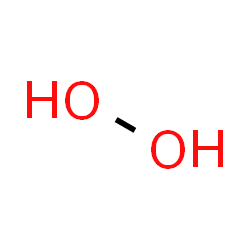
\includegraphics[width=3cm,scale=0.4]{img/763.png} \end{center} & 
             H: H271, H302, H314 e H332.
             
             P: P210, P220, P221, P260, P261, P264, P270, P271, P280, P283, P301+P312, P301+P330+P331, P303+P361+P353, P304+P312, P304+P340, P305+P351+P338, P306+P360, P310, P312, P321, P330, P363, P370+P378, P371+P380+P375, P405, e P501. & \begin{center} \begin{tabular}{cc}
                  
\includegraphics[scale=0.15]{img/pittogrammi/Flammable.png}&  
\includegraphics[scale=0.15]{img/pittogrammi/Explosive.png} \\
                  
\includegraphics[scale=0.15]{img/pittogrammi/Flammable.png}&  
\includegraphics[scale=0.15]{img/pittogrammi/Explosive.png} 
             \end{tabular}\end{center} & guanti, occhiali e visiera\\
    \bottomrule
    \end{tabularx}
    \caption{Tabella con i composti chimici utilizzati nell'esperienza, le frasi P e H vengono riportate per esteso al fondo della relazione.}
    \label{tab:tab1}
    \normalsize
\end{table}





Per i DPI sei costretto a cercare il nome del composto e scrivere di seguito scheda di sicurezza (es. acido benzoico scheda di sicurezza). Cerca di ricordarti il produttore, fai magari una foto in lab del contenitore, perchè possono variare. In fondo alla secheda trovi ache le info sui DPI oltre a altre varie info utili.

Altri siti utili che puoi utilizzare sono:
\begingroup
\begin{multicols}{2}
\begin{itemize}
    \item \href{https://molview.org/}{\textcolor{blue}{MolView}: sito ottimo per avere immagini 2D e 3D dei composti chimici;}
    \item \href{https://echa.europa.eu/it/regulations/clp/clp-pictograms}{\textcolor{blue}{ECHA}: per i simboli dei pittogrammi aiutati con questo se serve;}
    \item \href{https://echa.europa.eu/it/information-on-chemicals/cl-inventory-database}{\textcolor{blue}{ECHA}: per quanto riguarda le informazioni dei composti e la loro classificazione in europa;}
    \item \href{https://pubchem.ncbi.nlm.nih.gov/}{\textcolor{blue}{PubChem}: ottimo sito per informazioni generali dei composti chimici;}
    \item \href{http://www.chemspider.com/}{\textcolor{blue}{ChemSpider}: sito simile a PubChem;}
    \item \href{https://go.drugbank.com/}{\textcolor{blue}{DrugBank}}
    \item \href{https://www.ebi.ac.uk/chebi/init.do}{\textcolor{blue}{Chemical Entities of Biological Interest (ChEBI)}}
    \item \href{https://www.ebi.ac.uk/chembl/}{\textcolor{blue}{ChEMBL Database}}
    \item \href{https://commonchemistry.cas.org/}{\textcolor{blue}{CAS Common Chemistry}}
    \item \href{https://dguv.de/corona/index.jsp}{\textcolor{blue}{DGUV}}
    \item \href{https://www.rcsb.org/}{\textcolor{blue}{RCSB PDB}: Proteine DataBank}
    \item \href{https://www.efsa.europa.eu/it}{\textcolor{blue}{EFSA}: European Food Safety Authority}
    \item \href{http://eawag-bbd.ethz.ch/}{\textcolor{blue}{EAWAG BBD/PPS}: Biocatalysis/Biodegradation Database;}
    \item \href{https://sinu.it/}{\textcolor{blue}{SINU}: Società Italiana di Nutrizione;}
    \item \href{https://www.ars.usda.gov/}{\textcolor{blue}{ARS}: Agricultural Research Service;}
    \item \href{https://www.nist.gov/}{\textcolor{blue}{NIST}: National Istitute of Standards and Technology;}
    \item \href{https://www.rsc.org/merck-index}{\textcolor{blue}{The Merck Index Online}: For over 120 years The Merck Index has been regarded as the most authoritative and reliable source of information on chemicals, drugs and biologicals..}
\end{itemize}
\end{multicols}
\endgroup
\section{Procedimento}
Riferisce la procedura  operativa seguita. Spesso si completa con un disegno schematico dell'attrezzatura utilizzata, quando è utile per descrivere le istruzioni di assemblaggio della stessa. Qui devi spiegare in maniera sintetica ma esaustiva tutti i passaggi da te svolti durante l'esperimento.

Sono ammessi anche dei commenti o delle osservazioni, se hanno senso. Magari ti sei accorto che una reazione è particolarmente esotermica e la provetta diventa troppo calda da tenere in mano e allora puoi scrivere in corsivo, o con altri stratagemmi, perfar capire che questo parte esula dal procedimento ma che è un consiglio per la buona riuscita dell'esperimento.

es.
Aggiungere la lega di di Devarda. 
\textit{Attenzione! Dopo l'aggiunta il contenuto della provetta raggiunge alte temperature, meglio svolgere l'operazione vicino ad un bancone e con una scarabattola per posare la provetta.}


Un altra cosa che puoi aggiungere è un flowchart che riassuma i passaggi, questo può servirti a te in prima batutta per aver chiaro il procedimento e eventualmente studiare.
\begin{center}
    \vspace{0.5cm}
    \begin{tikzpicture}[node distance=2cm] % per guida -> https://it.overleaf.com/learn/latex/LaTeX_Graphics_using_TikZ%3A_A_Tutorial_for_Beginners_(Part_3)%E2%80%94Creating_Flowcharts
    \node (start) [startstop] {Inizio};
    \node (in1) [io, below of=start] {Ingresso};
    \node (pro1) [process, below of=in1] {Processo 1};
    \node (dec1) [decision, below of=pro1,  yshift=-0.5cm] {Decsione 1};
    \node (pro2a) [process, below of=dec1, yshift=-0.5cm] {Process 2a};
    \node (pro2b) [process, right of=dec1, xshift=2cm] {Process 2b};
    \node (out1) [io, below of=pro2a] {Output};
    \node (stop) [startstop, below of=out1] {Stop};
    
    \draw [arrow] (start) -- (in1);
    \draw [arrow] (in1) -- (pro1);
    \draw [arrow] (pro1) -- (dec1);
    \draw [arrow] (dec1) -- node[anchor=east] {yes} (pro2a);
    \draw [arrow] (dec1) -- node[anchor=south] {no} (pro2b);
    \draw [arrow] (pro2b) |- (pro1); %per fare linea segmentata
    \draw [arrow] (pro2a) -- (out1);
    \draw [arrow] (out1) -- (stop);
    \end{tikzpicture}
\end{center}

\section{Dati e Calcoli}
In questa sezione devi raccolgiere tutti i risultati che hai ottenuto. Vanno bene  foto, tabelle di dati e osservazioni personali. I dati sarebbe buono che vengano raccolti in tabella se sono in numero sufficiente. \'E acneh vero che puoi unire le due sezioni dei dati per rendere più discorsivo il tutto, a tua scelta.

In questa sezione devi anche scrivere tutte le formule che usi per i calcoli indicando cosa servono le formule e le loro unità di misura.

Ci sono due modi per impostare le cose, nel primo modo scrivi prima tutte le formule e poi dopo svilgi i conti con i tuoi dati, oppure scrivi la formula e poi subito dopo il tuo calcolo. Sta a te scegliere. (Se vuoi fare il secondo metodo si potrebbe usare una tabella

Primo metododo:
Le moli si trovano tramite la seguente formula:
\begin{equation}
   n=M[mol/L]\cdot V[L]=n [mol] 
   \label{eq:mol} %questo ti serve per citare le equazioni, in questa sezione non è molto utile ma nei cenni teorici ti può aiutare a scrivere meglio le frasi senza intortarti da solo
\end{equation}
E ora si svolge il calcolo sui propri dati, in questo caso aggiungo un "*" all'ambiente per togliere i numeri:
\begin{equation*}
   n=\frac{0.5\cdot 25}{1000}=0.0125 [mol] 
\end{equation*}
Si divide per  1000 percheè il volume è stato espresso in mL

Nel secondo modo invece:
\begin{center}
    \begin{tabularx}{0.9\textwidth}{XcX}
    Formule & & Calcoli\\
    \midrule
    $n=M[mol/L]\cdot V[L]=n [mol] $ &$\rightarrow$& $ n=\frac{0.5\cdot 25}{1000}=0.0125 [mol] $\\
    $n=M[mol/L]\cdot V[L]=n [mol] $ &$\rightarrow$& $ n=\frac{0.5\cdot 25}{1000}=0.0125 [mol] $\\
    $n=M[mol/L]\cdot V[L]=n [mol] $ &$\rightarrow$& $ n=\frac{0.5\cdot 25}{1000}=0.0125 [mol] $\\
    $n=M[mol/L]\cdot V[L]=n [mol] $ &$\rightarrow$& $ n=\frac{0.5\cdot 25}{1000}=0.0125 [mol] $\\
    $n=M[mol/L]\cdot V[L]=n [mol] $ &$\rightarrow$& $ n=\frac{0.5\cdot 25}{1000}=0.0125 [mol] $\\
    \end{tabularx}
\end{center}
Bisogna trovare il modo per distanziare un po' il testo in verticale ma ci può stare.
Io preferisco il primo metodo perchè da più spazio.


\subsection{Dati sperimentali}
Vanno riportati \textit{tutti} i dati sperimentali, evidenziando se necessario, quelli "aberranti", cioè da scartare sulla base si un analisi statistica. Laddove possibile, è bene raccogliere i dati sotto forma di tabelle.
\vspace{1ex}
\begin {center}
\begin{tabular}{c|c}
     Esperimento &  Risultato\\
     1 & 10\\
     2 & 15\\
     3 & ...
\end{tabular}
\end {center}

\subsection{Elaborazione dei dati}
(se necessario anche grafica): riporta i calcoli effettuati a partire dai risultati sperimentali, indicando le relazioni matematiche utilizzate. L'eleaborazione può consistere anche nella costruzione di diagrammi o grafici. A volte essa prevede anche il trattamento statistico dei dati.
Plotting from data:
\begin{center}
\vspace{2ex}
\begin{figure}[!ht]
    \centering
    \begin{tikzpicture}
        \begin{axis}[
            title={Temperature dependence of CuSO\(_4\cdot\)5H\(_2\)O solubility},
            xlabel={Temperature [\textcelsius]},
            ylabel={Solubility [g per 100 g water]},
            xmin=0, xmax=100,
            ymin=0, ymax=120,
            xtick={0,20,40,60,80,100},
            ytick={0,20,40,60,80,100,120},
            legend pos=north west,
            ymajorgrids=true,
            grid style=dashed,
            ]

            \addplot[
                color=blue,
                mark=square,
                ]
                coordinates {
                (0,23.1)(10,27.5)(20,32)(30,37.8)(40,44.6)(60,61.8)(80,83.8)(100,114)
                };
                \legend{CuSO\(_4\cdot\)5H\(_2\)O}
                
            \end{axis}
        \end{tikzpicture}
    \caption{Grafico di solubilità del solfato di rame in base alla temperatura.}
    \label{plt:1}
\end{figure}

\end{center}
\newpage


\section{Conclusioni}
Qui trovano spazio eventuali note dell'operatore riguardanti aspetti procedurali e la sua valutazione dei risultati precedentemente elaborati, in riferimento agli obiettivi previsti dall'esperienza. \'E importante segnalare eventuali anomalie riscontrate nei confronti della metodica utilizzata, nonchè i passaggi che hanno causato difficoltà (in particolare sotto il profilo di sicurezza).

Ultima sezione della relazione, forse è la più importante insieme ad obbiettivo e procedimento. In questa parte devi trare le conclusioni dell'esperimento. 
\begin{itemize}
    \item Esito (riuscito-fallito)
    \item Risultato (sensato-assurdo)
    \item Osservazioni tue personali sui passaggi che potresti aver sbagliato o che magari ritieni di aver fato nella maniera migliore rispetto alle indicazioni del prof, spiegare e motivare.
\end{itemize}
\section{Bibliografia}
Alle superiori non serve ma in futuro, se continui, sarà essenziale citare le fonti che hai usato per stendere un qualsiasi tipo di elaborato scritto ( ad eccezione del materiale del docente). Questa sezione serve proprio a quello, ti permette di raccogliere i siti e gli articoli da cui hai preso le informazioni (soprattutto quelle dei cenni teorici). 

Ti può servire, nel caso tu volessi recuperare le fonti da cui hai preso le cose per studiare o nel caso qualcuno ti dicesse che hai sbagliato a scrivere qualcosa.

Esempio di citazione.\autocite{einstein}

\printbibliography %Prints bibliography
\endgroup
%stanno onguno su pagine diverse
\section*{\quad \   Frasi H e P}
Trovi ai seguenti link, \href{https://it.wikipedia.org/wiki/Indicazioni_di_pericolo_H}{\textcolor{blue}{H}} e \href{https://it.wikipedia.org/wiki/Consigli_P}{\textcolor{blue}{P}}, le frasi P e H che dovrai aggiungerti in modo da avere già la lista fatta una volta per tutte e poi per ogni relazione togli quelle che non ti servono.

\begingroup
\begin{multicols}{2}
\scriptsize
\subsection*{Pericoli fisici}
\begin{itemize}
    \item \Hphrase{H200}
    \item \Hphrase{H240}
\end{itemize}
\subsection*{Pericoli per la salute}
\begin{itemize}
    \item \Hphrase{H315}
    \item \Hphrase{H318}
    \item
\end{itemize}
\subsection*{Consigli di prudenza di carattere generale}
\begin{itemize}
    \item \Pphrase{P101}
    \item
\end{itemize}
\end{multicols}
\endgroup



\newpage
\section*{Esempi}
\textbf{Qui trovi alcune prove ed esempi di come mettere le immagini.}

\begin{figure}[h]
    \centering
    \begin{subfigure}[]{0.5\linewidth}
    \centering
    
\includegraphics[scale=0.2]{img/pittogrammi/Acute toxicity.png}
    \caption{Acute toxicity}
    \end{subfigure}
    \begin{subfigure}[]{0.5\linewidth}
    \centering
    
\includegraphics[scale=0.2]{img/pittogrammi/Explosive.png}
    \caption{Explosive}
    \end{subfigure}
    \caption{Due immagini incolonnate al centro della pagina con posizione h definita da te.}
    \label{fig:1}
\end{figure}

\textit{Lorem ipsum dolor sit amet, consectetur adipiscing elit. Maecenas eget nisl elementum, pretium libero suscipit, interdum tellus. Praesent luctus commodo massa, vel molestie augue laoreet ac. Phasellus sodales auctor erat eu porta. Donec at volutpat nunc. Phasellus pretium, eros vitae cursus ornare, turpis massa egestas sem, ut varius ipsum metus nec mi. Integer ut odio erat. Interdum et malesuada fames ac ante ipsum primis in faucibus. Sed finibus, tortor in tristique iaculis, odio tortor finibus nisi, nec varius felis justo eu tortor. Interdum et malesuada fames ac ante ipsum primis in faucibus. Donec ultrices in ante vel imperdiet. Ut porttitor consectetur sodales. Vestibulum ante ipsum primis in faucibus orci luctus et ultrices posuere cubilia curae; Nullam non neque quis tortor convallis pulvinar id vel libero.}

\begin{figure}[!h]
\floatbox[{\capbeside\thisfloatsetup{capbesideposition={right,top},capbesidewidth=0.45\textwidth}}]{figure}[\FBwidth]
{\caption{didascalia dell'immagine centrale con didascalia a fianco.}}
{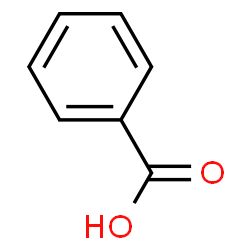
\includegraphics[width=0.1\textwidth]{img/acbenz.png}}
{\label{fig:2}}
\end{figure}

\textit{Aliquam erat nulla, suscipit id dignissim molestie, eleifend quis tortor. Pellentesque tempus egestas orci, sit amet eleifend elit condimentum id. Etiam id nisi velit. Etiam mauris nisl, facilisis sed egestas nec, tempor a est. In eget lacus vitae velit volutpat maximus. Vestibulum maximus arcu sit amet lacus maximus consequat. Duis sodales libero non metus finibus, eget ornare sem consequat.}

\begin{wrapfigure}{r}{0.3\textwidth} %this figure will be at the right
    \centering
    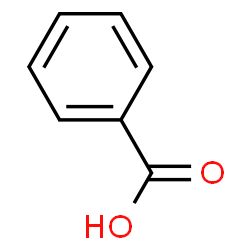
\includegraphics[scale=0.5]{img/acbenz.png}
    \caption{Didascalia dell'immagine sulla destra circondata da testo.} 
    \label{fig:3}
\end{wrapfigure}

\textit{Nullam vel lorem porttitor, convallis ex eget, condimentum velit. Integer sed sem aliquet, elementum ipsum in, rutrum elit. Vestibulum in arcu eget odio egestas varius. Vivamus lacus augue, dignissim at arcu a, consequat iaculis leo. Nam sit amet varius tellus. Nulla tempor velit nibh, et tincidunt diam porta vel. Mauris sit amet erat ut neque vehicula ultrices et eu sem. Phasellus pellentesque ultricies sapien. Curabitur at sodales mauris, maximus auctor mi. Vestibulum semper mauris in euismod rutrum. Fusce pellentesque in mi ac euismod.}

\textit{Nam gravida magna ut volutpat placerat. Pellentesque habitant morbi tristique senectus et netus et malesuada fames ac turpis egestas. Sed consequat justo condimentum metus bibendum mattis. Etiam id euismod ante. Nam sit amet ex libero. Proin id mauris at neque pellentesque accumsan eu ut ligula. Vivamus sodales magna sed risus faucibus tincidunt in eu felis.}

\begin{figure}
    \centering
    
\includegraphics[scale=0.2]{img/pittogrammi/Acute toxicity.png}
    
\includegraphics[scale=0.2]{img/pittogrammi/Explosive.png}
    \caption{Figure affiancate al centro della pagina nella posizione decisa da LaTex}
    \label{fig:4}
\end{figure}

\textit{Vivamus sit amet suscipit turpis, at eleifend risus. Vestibulum ante ipsum primis in faucibus orci luctus et ultrices posuere cubilia curae; Curabitur eget pharetra est, in mattis erat. Aenean pharetra finibus posuere. Nullam ipsum lacus, molestie nec eros eu, lacinia facilisis augue. Aenean dapibus rhoncus mi ut vulputate. Mauris commodo ultricies nulla egestas porttitor.}

\begin{figure}[h]
    \centering
    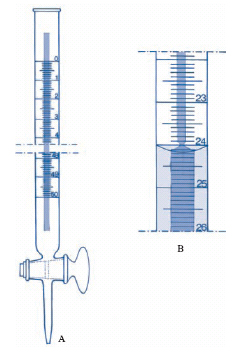
\includegraphics{img/buretta.jpg}
    \caption{Buretta}
    \label{fig:5}
\end{figure}









\end{document}
